\documentclass[12pt,a4paper]{ctexart}

\usepackage[UTF8]{ctex}
\usepackage{geometry}
\usepackage{graphicx}
\usepackage{xcolor}
\usepackage{tikz}
\usepackage{fontspec}
\usepackage{setspace}
\usepackage{enumitem}
\usepackage{booktabs}
\usepackage{array}
\usepackage{longtable}
\usepackage{hyperref}
\usepackage{fancyhdr}
\usepackage{titlesec}
\usepackage{multicol}
\usepackage{xurl}
\usepackage{tocloft}

\renewcommand{\cfttoctitlefont}{\hfill\bfseries\Large}
\renewcommand{\cftaftertoctitle}{\hfill}
\geometry{left=2.5cm,right=2.5cm,top=2.5cm,bottom=2.5cm}

\definecolor{black}{RGB}{0,0,0}
\definecolor{mainblue}{RGB}{0,82,147}
\definecolor{accentgold}{RGB}{180,140,60}
\definecolor{lightgray}{RGB}{245,245,245}
\definecolor{darkgray}{RGB}{80,80,80}
\definecolor{mainred}{RGB}{230,1,45}

\hypersetup{
    colorlinks=true,
    linkcolor=black,
    urlcolor=mainblue,
    citecolor=mainblue,
    pdfborder={0 0 0}
}

\pagestyle{fancy}
\fancyhf{}
\fancyhead[L]{\small\color{darkgray}\textbf{量子行业每周新闻洞察}}
\fancyhead[R]{\small\color{darkgray}\textbf{总第186期}}
\fancyfoot[C]{\thepage}
\renewcommand{\headrulewidth}{0.4pt}
\renewcommand{\footrulewidth}{0pt}

\titleformat{\section}
    {\Large\bfseries\color{mainred}}
    {\thesection、}{0em}{}
\titleformat{\subsection}
    {\large\bfseries\color{mainred}}
    {\thesubsection、}{0em}{}

\newcolumntype{L}[1]{>{\raggedright\arraybackslash}p{#1}}
\newcolumntype{C}[1]{>{\centering\arraybackslash}p{#1}}

\begin{document}

% ==================== 封面 ====================
\begin{titlepage}
\begin{tikzpicture}[remember picture,overlay]
    \fill[mainred] ([yshift=-0.5cm]current page.north west) rectangle ([yshift=-1.2cm]current page.north east);
    \fill[mainred] ([yshift=1.2cm]current page.south west) rectangle ([yshift=0.5cm]current page.south east);
\end{tikzpicture}

\vspace*{4cm}

\begin{center}
    {\fontsize{44}{52}\selectfont\bfseries\color{black} \textbf{量子行业每周新闻洞察}}

    \vspace{0.8cm}

    {\fontsize{16}{22}\selectfont\color{darkgray} 2026.06.28 — 2026.07.03 }
    {\fontsize{16}{22}\selectfont\color{darkgray} \textbf{WEEKLY NEWS}}

    \vspace{1.5cm}

    {\fontsize{20}{26}\selectfont\color{mainred}\textbf{（总第\textbf{ 186 }期）}}

    \vspace{4cm}

    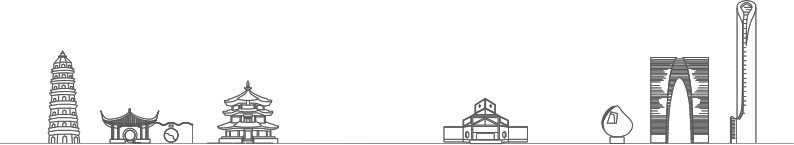
\includegraphics[width=\textwidth]{Cover_Suzhou.png}

    \vfill

    {\fontsize{12}{16}\selectfont\color{darkgray} 量子科技长三角产业创新中心\\编制：战略情报与成果专利室、产业发展部（理事会办公室）}
\end{center}
\end{titlepage}

% ==================== 目录 ====================
\pagenumbering{roman}
\newpage
\tableofcontents

\newpage

% ==================== 摘要 ====================
\pagenumbering{arabic}
\setcounter{page}{1}
\begin{center}
{\Large\bfseries\color{mainred} 摘\hspace{2em}要}
\end{center}
\addcontentsline{toc}{section}{摘要}


\textbf{ 宏观态势：}

全球量子科技竞争已进入战略落地的关键阶段。各国正从技术研发向实际部署和应用迁移加速迈进，俄罗斯、丹麦、欧洲在量子光源、通信网络及传感领域取得具体进展；韩国将量子列为国家战略技术并斥巨资投入，印度则在核心硬件上实现突破。同时，量子安全成为紧迫议题，微软设定后量子密码迁移时间表，多国启动专项人才培养。从金融、国防到汽车行业，深度合作与路线图发布表明，量子技术的产业化应用正从探索转向战略性布局。


\textbf{ 科技前沿：}

前沿研究正聚焦于提升量子技术的实用性与可扩展性。高质量单光子源领域取得显著进展，包括利用二维材料与实现室温即插即用方案，这为可部署的量子通信网络铺平道路。在计算与模拟方面，科研人员借助现有量子硬件探索粒子物理等超越经典算力的场景，并开发新算法模拟噪声量子电路。此外，量子网络中的量子态分布式生成以及离散时空晶体的发现，预示着更复杂的网络架构和全新量子光学器件的可能性。


\textbf{ 产品动态：}

量子计算产品正从实验室走向商业化、平台化与生态化。混合量子云平台成为主流交付模式，在韩国、欧洲等地开始商用或试点，旨在简化硬件接入。软件生态愈发成熟，重点在于与高性能计算的融合及跨平台集成，如多个量子编译框架与英伟达平台对接。系统架构创新同样活跃，致力于通用光子计算和分布式量子编译。这些动态表明，行业正通过构建易用的开发环境与安全解决方案，降低量子技术的应用门槛。


\textbf{ 企业资讯：}

产业链企业正加速构建生态壁垒并拓展全球市场。韩国通信巨头将量子安全重心从量子密钥分发扩展至后量子密码，着力推动全面商业化。硬件与软件公司通过跨界合作，在加拿大、美国等地共建集成技术中心，打通光子封装、量子控制与AI集成等关键环节。金融机构开始入局探索衍生品定价应用，而企业通过上市、组建新团队等方式为扩张蓄力，标志着量子产业正步入深度整合与规模化发展的前夜。


\textbf{ 资本运作：}

资本市场对量子技术的支持持续升温，并呈现多元化和理性化趋势。融资覆盖从早期硬件研发到成熟技术商业化的全周期，表明投资重心正向可落地场景倾斜。企业并购获监管批准，行业整合开始提速。同时，围绕核心技术成立的专项新公司，意在通过估值背书抢占市场高地。从政府科研资助到公司上市规划，资金正有效驱动量子测量、硬件及前沿容错计算等关键领域加速发展。






% ==================== 会议列表 ====================
{
    \newpage
    \section*{ 7月量子科技行业国内、国际会议}
    \addcontentsline{toc}{section}{ 7月量子科技行业国内、国际会议}
    \scriptsize
    \begin{longtable}{C{0.8cm}L{2.5cm}L{3cm}L{7cm}}
        \toprule[1.5pt]
        \textbf{序号} & \textbf{日期} & \textbf{地点} & \textbf{会议名称} \\
        \midrule
        \endfirsthead
        \toprule
        \textbf{序号} & \textbf{日期} & \textbf{地点} & \textbf{会议名称} \\
        \midrule
        \endhead
        \bottomrule
        \endfoot
        
        1 & 7月1日-3日 & 奥尔堡, 丹麦 & IEEE量子控制、计算与学习国际会议（IEEE qCCL 2026） \\
        \midrule[0.05pt]
        
        2 & 7月1日-3日 & 首尔, 韩国 & 2026量子信息会议（CQI 2026） \\
        \midrule[0.05pt]
        
        3 & 7月1日-3日 & 爱丁堡, 英国 & 2026青年量子研究者暑期学校 \\
        \midrule[0.05pt]
        
        4 & 7月2日-4日 & 首尔, 韩国 & Quantum Korea 2026 \\
        \midrule[0.05pt]
        
        5 & 7月6日-8日 & 海尔布隆, 德国 & 自然科学容错量子计算研讨会（FTQC4NSc） \\
        \midrule[0.05pt]
        
        6 & 7月6日-10日 & 那不勒斯, 意大利 & 第12届单光子研讨会（SPW 2026） \\
        \midrule[0.05pt]
        
        7 & 7月7日-10日 & 加尔各答, 印度 & 2026年IEEE量子计算国际研讨会：电路、系统、自动化与应用（QC-CSAA） \\
        \midrule[0.05pt]
        
        8 & 7月12日-17日 & 马斯特里赫特, 荷兰 & 量子传感与计量学（QSM） \\
        \midrule[0.05pt]
        
        9 & 7月13日-17日 & 代尔夫特, 荷兰 & 第7届自旋量子信息处理会议（Spin Qubit 7） \\
        \midrule[0.05pt]
        
        10 & 7月13日-17日 & 悉尼, 澳大利亚 & IEEE量子软件国际会议（QSW 2026） \\
        \midrule[0.05pt]
        
        11 & 7月16日-18日 & 波尔图, 葡萄牙 & 量子信息、计算、通信与模拟国际会议（QUANTICS 2026） \\
        \midrule[0.05pt]
        
        12 & 7月19日-23日 & 博尔德, 美国 & 有限温度非平衡超流体系统研讨会（FINESS 2026） \\
        \midrule[0.05pt]
        
        13 & 7月20日-24日 & 埃朗根, 德国 & 第30届中欧量子光学研讨会（CEWQO 2026） \\
        \midrule[0.05pt]
        
        14 & 7月22日-23日 & 芝加哥, 美国 & 全球量子论坛（GQF 2026） \\
        \midrule[0.05pt]
        
        15 & 7月25日-26日 & 伊斯顿, 美国 & 量子科学研讨会（Gordon Research Seminar） \\
        \midrule[0.05pt]
        
        16 & 7月26日-31日 & 伊斯顿, 美国 & 多体量子系统：量子计算、模拟、传感与新兴平台（Gordon Research Conference） \\
        \midrule[0.05pt]
        
        17 & 7月26日-8月1日 & 布拉格, 捷克共和国 & 量子与介观热力学前沿2026（FQMT'26） \\
        \midrule[0.05pt]
        
        18 & 7月27日-31日 & 科莫湖, 意大利 & 超快量子光学新前沿暑期学校 \\
        \midrule[0.05pt]
        
        19 & 7月27日-31日 & 艾哈迈达巴德及线上, 印度 & 自由空间量子通信短课程 \\
        \midrule[0.05pt]
        
    \end{longtable}
}




% ==================== 宏观态势 ====================
\newpage
\section{宏观态势}
\vspace{-0.5em}
\noindent\rule{\linewidth}{1.5pt}

\subsection{ 俄罗斯首次成功研制出芯片级压缩光量子光源，将研发基于该技术的量子计算系统 }

2026年07月03日消息，俄罗斯国家原子能公司...【近日宣布】→删除“近日”。开头有“2026年07月03日消息，”，后面没有重复日期词。修正后：2026年07月03日消息，俄罗斯国家原子能公司旗下俄罗斯量子中心研究团队宣布，已在芯片上制成...（删除“近日”）于压缩光的量子计算系统研发。团队下一步计划包括启动基于“压缩光”的量子计算系统研发，并把相关成果用于探测器和生物探测器制造。

\noindent\textbf{报道链接：}\url{https://en.iz.ru/en/2125548/2026-07-02/rosatom-announced-development-compressed-light-technology-scientists}

\subsection{ 澳大利亚Pawsey启动PULSE计划，12个超级计算与量子计算项目获支持 }

2026年07月03日消息，澳大利亚Pawsey...【近日启动】→删除“近日”。修正：2026年07月03日消息，澳大利亚Pawsey超级计算研究中心启动新一轮PULSE合作计划...究工作流程并访问先进的计算环境，推动量子计算等新兴算力进入更广泛的科研场景。Pawsey表示，这些项目将共同展示国家研究基础设施如何帮助澳大利亚研究人员突破计算可能性的界限。

\noindent\textbf{报道链接：}\url{https://pawsey.org.au/pulse-accelerates-australian-research/}

\subsection{ 丹麦建成新型量子通信网络，已连接多个政府部门实现安全通信 }

2026年07月03日消息，由丹麦量子通信基础设施项目...【于昨日正式投入运营】→删除“昨日”。修正：2026年07月03日消息，由丹麦量子通信基础设施项目QCI.DK开发的一条量子通信网络正式投入运营...子态生成密钥的量子密钥分发技术，并使用连续变量方案，可在现有光纤通信网络上运行而无需改造。项目团队表示，后续将通过欧洲EuroQCI计划把量子安全连接扩展至瑞典和波兰，相关技术也正由DTU孵化企业Celare Quantum Communications推进商业化。

\noindent\textbf{报道链接：}\url{https://www.dtu.dk/english/news/all-news/new-quantum-communication-network-protects-data-now-and-in-the-future?id=83129c45-491d-4a56-beea-62c806f72bb9}

\subsection{ 欧洲CARIOQA-PMP研究项目探索量子传感助力卫星重力测量 }

2026年07月01日消息，欧洲CARIOQA-PMP项目【近日介绍】→删除“近日”。修正：2026年07月01日消息，欧洲CARIOQA-PMP项目介绍了一项关于未来卫星重力任务的研究...Geophysical Journal International》的论文认为，这类量子化任务设计有望带来更高灵敏度和更丰富的信息，有望为下一代空间量子测量、重力遥感和地球科学任务提供技术依据。

\noindent\textbf{报道链接：}\url{https://carioqa-quantumpathfinder.eu/carioqa-pmp-highlights-new-research-on-quantum-gravity-measurements-from-space/}

\subsection{ 法国农业信贷银行与中性原子量子计算公司Pasqal深化合作伙伴关系 }

2026年07月01日消息，法国农业信贷银行与中性原子量子计算公司Pasqal【昨日宣布签署】→删除“昨日”。修正：2026年07月01日消息，法国农业信贷银行与中性原子量子计算公司Pasqal宣布签署一份战略合作协议...例。据介绍，双方此前已在交易对手信用违约风险评估和投资组合优化方面开展项目，结果显示特定条件下量子算法有望优于经典方法。新合作的下一阶段将聚焦于监控与风险加权资产相关的资本准备金消耗。

\noindent\textbf{报道链接：}\url{https://www.pasqal.com/newsroom/credit-agricole-cib-and-pasqal-advance-their-strategic-partnership-to-deploy-quantum-computing-applied-to-finance/}

\subsection{ 韩国将量子列为国家十大战略技术，五年总研发将投入超200万亿韩元 }

2026年07月01日消息，韩国科技与信息通信技术部【近日表示】→删除“近日”。修正：2026年07月01日消息，韩国科技与信息通信技术部表示，该国政府已敲定2026至2030年第六个科学技术基本规划...万亿韩元，其中60万亿韩元投向人工智能、半导体、先进生物、量子科技等10大领域的55项技术。据悉，该规划文件未单列量子专项预算，但将量子纳入了长期经济与国家安全议程，而非狭隘的研究项目。

\noindent\textbf{报道链接：}\url{https://thequantuminsider.com/2026/06/30/south-korea-commits-200-trillion-won-to-rd-quantum-listed-as-strategic-tech/}

\subsection{ 微软宣布将于2029年前推动关键产品和服务迁移至后量子密码学 }

2026年07月02日消息，微软【近日宣布】→删除“近日”。修正：2026年07月02日消息，微软宣布其正在加快量子安全路线图...管当前量子计算机尚不足以破解现代加密，但“先窃取、后解密”风险已迫使机构提早准备，因此其计划在“Quantum Safe Program”框架下，于2029年前推动关键产品和服务迁移至后量子密码学（PQC），并把量子安全要求纳入其安全未来倡议。

\noindent\textbf{报道链接：}\url{https://www.microsoft.com/en-us/security/blog/2026/06/30/microsoft-advances-quantum-safe-security-as-the-risk-timeline-shifts/}

\subsection{ 美国两大政府机构联合启动QuantumEagle计划 以推动该国量子计算生态系统发展 }

2026年07月02日消息，美国国家安全局（NSA）物理科学实验室和美国陆军作战能力发展司令部（DEVCOM）陆军研究办公室宣布联合启动一项名为QuantumEagle的计划，没有模糊时间词，也不需要删除重复日期。开头是“2026年07月02日消息，美国国家安全局...”，后面没有类似日期。无需修正。业创新和增长的五大关键领域：行业参与、商业路线图、供应链进步、 算法应用和基础研究。该新计划旨在推动美国量子计算生态系统的发展，并巩固美国在量子技术领域的领导地位。

\noindent\textbf{报道链接：}\url{https://www.nsa.gov/Press-Room/Press-Releases-Statements/Press-Release-View/Article/4529557/nsa-devcom-army-research-office-launch-quantumeagle-initiative/}

\subsection{ SEALSQ发布面向汽车行业的后量子安全芯片路线图 }

2026年07月02日消息，SEALSQ公司【近日公布】→删除“近日”。修正：2026年07月02日消息，SEALSQ公司公布了其面向下一代汽车的安全路线图...未来量子威胁。SEALSQ称，它将依托内部ASIC设计服务，为OEM厂、一级供应商和半导体制造商提供可信平台模块、安全微控制器、嵌入式HSM IP、基于芯片组的硬件安全模块以及定制抗量子ASIC等产品，目标是在不重新设计核心硅架构的前提下，为汽车系统加入抗量子信任根。

\noindent\textbf{报道链接：}\url{https://www.globenewswire.com/news-release/2026/07/01/3320677/0/en/sealsq-to-bring-post-quantum-security-to-the-automotive-industry.html}

\subsection{ 印度与美国宣布在人工智能、量子技术等领域深化合作伙伴关系 }

2026年07月01日消息，印度与美国【近日宣布】→删除“近日”。修正：2026年07月01日消息，印度与美国宣布在半导体、人工智能、量子技术及关键矿产领域深化合作...阶段。印度驻美大使表示，印度在半导体、AI和量子技术方面采取使命导向模式，结合美国的创新生态，能够构建可信且富有韧性的技术生态系统，同时能确保支撑新兴技术的关键基础设施安全可控。

\noindent\textbf{报道链接：}\url{https://indiawest.com/india-us-advance-ai-chip-and-quantum-cooperation/}

\subsection{ 印度量子技术新里程碑：国产稀释制冷机实现4开尔文极低温环境运行 }

2026年07月01日消息，印度阿马拉瓦蒂量子谷【近日宣布】→删除“近日”。修正：2026年07月01日消息，印度阿马拉瓦蒂量子谷宣布，其量子基础设施内一套以本土组件为主的稀释制冷机已实现4开尔文...子传感器、低温电子学和单光子探测器等提供测试与表征条件。业内认为，这一进展将减少印度量子硬件研发对海外低温测试平台的依赖，并支撑其国家量子任务下的本土量子计算、量子通信和先进传感生态建设。

\noindent\textbf{报道链接：}\url{https://www.bignewsnetwork.com/news/279140295/amaravati-quantum-valley-reaches-4-kelvin-at-quantum-reference-facility-using-indian-made-components}

\subsection{ 韩国启动后量子密码培训计划，年内培养620名专业人员 }

2026年07月01日消息，韩国科学技术信息通信部与韩国互联网振兴院（KISA）【近日宣布】→删除“近日”。修正：2026年07月01日消息，韩国科学技术信息通信部与韩国互联网振兴院（KISA）宣布，他们将于7月至11月开设后量子密码专业培训项目...践课招收440人，总计培养620名专业人员。此举与韩国推进国家密码体系向后量子密码过渡、发展量子科技与量子产业的综合规划相衔接，显示其正从政策与人才两端加快量子安全基础能力建设。

\noindent\textbf{报道链接：}\url{https://www.digitaltoday.co.kr/en/view/76452/science-ministry-to-push-professional-training-in-post-quantum-cryptography}

\subsection{ 美国查塔努加量子合作组织启动量子预学徒培训计划 }

2026年06月29日消息，美国田纳西州查塔努加量子合作组织（CQC）【近日从17家田纳西雇主中遴选】→删除“近日”。修正：2026年06月29日消息，美国田纳西州查塔努加量子合作组织（CQC）从17家田纳西雇主中遴选出18名专业人士...者而扩至18人。每位学员将完成一项“量子机遇评估”结业项目，以评估与其雇主相关的潜在用例和未来应用

\noindent\textbf{报道链接：}\url{https://www.chattanoogaquantum.com/resources/tennessee-employers-join-nations-first-quantum-pre-apprenticeship-to-prepare-for-emerging-technology-opportunities}

\subsection{ 量子计算平民化：欧洲EuroHPC JU启动量子系统接入试点 }

2026年06月29日消息，欧洲高性能计算联合体（EuroHPC JU）【近日宣布】→删除“近日”。修正：2026年06月29日消息，欧洲高性能计算联合体（EuroHPC JU）宣布，即日起欧洲用户可通过新启动的EuroHPC量子接入试点项目...问欧洲日益完善的量子计算基础设施。EuroHPC JU采取了混合策略，将量子计算机与欧洲顶尖超级计算基础设施集成，以实现量子加速的高性能计算，并已投资一系列互补的量子技术，包括离子阱、超导电路、光子学、中性原子和绝热（退火）系统。首批通过该试点项目开放的系统包括：基于超导量子比特的Euro-Q-Exa、基于光子量子比特的Lucy、基于离子阱的Piast-Q以及基于超导量子比特的VLQ，首个申请截止日期为2026年8月1日。

\noindent\textbf{报道链接：}\url{https://www.eurohpc-ju.europa.eu/eurohpc-ju-opens-access-its-quantum-computers-2026-06-25\_en?utm\_source=chatgpt.com}

\subsection{ 德国SPRIND启动量子传感计划，欲加速量子技术从实验室走向市场 }

2026年06月29日消息，德国联邦突破性创新机构SPRIND【近日启动】→删除“近日”。修正：2026年06月29日消息，德国联邦突破性创新机构SPRIND启动“量子传感计划”...技术走向实际应用，支持其进入市场，并强化欧洲在量子技术这一最具潜力领域的生态系统。SPRIND正以“SPRIND Funken”挑战式资助项目为开端，推出两大资助方向：“量子驱动智能”专注于将量子传感器数据与现有数据源、模型及传感器系统结合，生成可操作的洞察；“量子感知探索”则致力于拓展量子传感的技术基础。

\noindent\textbf{报道链接：}\url{https://thequantuminsider.com/2026/06/24/sprind-launches-quantum-sensing-initiative-to-back-european-projects-and-startups/}

\subsection{ 量子计算转向战略准备：IBM新报告揭示行业应用新趋势与挑战 }

2026年06月30日消息，IBM商业价值研究院【最近发布】→“最近”也是模糊时间词，删除。修正：2026年06月30日消息，IBM商业价值研究院发布名为《量子优势之旅》的报告指出...发现，先行者关注的重点已不再是抽象基准，而是在航空航天、金融、能源、生命科学和制造业等领域的实际应用案例。IBM指出，技能短缺、技术尚不成熟以及时间表不确定是主要障碍，同时强调合作与生态系统建设正成为量子准备工作的核心。

\noindent\textbf{报道链接：}\url{https://thequantuminsider.com/2026/06/21/the-path-to-quantum-advantage-is-built-on-readiness-not-hype-ibm-report-suggests/}

\subsection{ 欧洲量子增强应用卓越中心成立，19家合作伙伴携手打造一站式量子计算服务平台 }

2026年06月29日消息，欧洲【近日启动】→删除“近日”。修正：2026年06月29日消息，欧洲启动了一个名为“量子增强应用卓越中心（QEC4QEA）”的新倡议...企业（EuroHPC JU）资助，欧盟出资约490万欧元，为期四年，致力于将前沿量子研究转化为实用工业解决方案。QEC4QEA由德国于利希超算中心协调，汇聚了来自西班牙（ICFO）、德国、意大利、法国等19家学术与产业合作伙伴，旨在打造一个简化访问量子增强技术与服务的统一平台（即一站式中心)。该计划的核心是将量子能力集成到经典高性能计算（HPC）工作流中，期望在计算复杂性成为瓶颈的领域提升效率，如高级密码学与数据安全、金融建模与碰撞预测、机器学习与图像分析等。

\noindent\textbf{报道链接：}\url{https://www.icfo.eu/news/2683/quantum-excellence-centre-for-quantum-enhanced-applications/880/}

\subsection{ QuEra Computing公布下一代量子系统，目标实现千倍性能飞跃与十亿次逻辑运算 }

2026年06月29日消息，QuEra Computing【近日在其路线图网络研讨会后，公布】→删除“近日”。修正：2026年06月29日消息，QuEra Computing在其路线图网络研讨会后，公布了其下一代容错量子计算系统细节。注意“近日”在开头，删除。起解决方案征集活动，邀请企业、高性能计算中心及政府机构提交其最具价值的难题作为潜在应用场景。该下一代系统预计于2028至2029年间在QuEra内部率先部署，相比其首台容错量子计算机“Libra”，性能提升约千倍。据规划，新系统将拥有超过1000个逻辑量子比特、10⁻9的逻辑错误率，并在单个处理核心中集成超过20000个物理量子比特。

\noindent\textbf{报道链接：}\url{https://www.quera.com/press-releases/quera-unveils-gigaquop-class-fault-tolerant-roadmap-and-invites-organizations-to-co-design-quantum-applications}

\subsection{ 费米实验室与Qblox达成合作，加速在美推进量子控制平台商业化及人才培养 }

2026年06月29日消息，美国能源部技术商业化办公室【近日宣布】→删除“近日”。修正：2026年06月29日消息，美国能源部技术商业化办公室宣布，费米国家加速器实验室（Fermilab）已与荷兰量子控制硬件公司Qblox签署正式协议。，并以此平台为基础建立针对性人才培养计划。QICK由费米实验室开发，是一款用于管理量子读出与控制的开源平台，它在同步量子处理器与传感器发面发挥着关键作用，被视为支撑量子生态的基础技术。合作中，Qblox将主导两大方向：一是供应链商业化，协调QICK的制造、分销与商业化，构建本土化量子供应链；二是人才建设，利用QICK开发教育培训项目，为美国量子行业培养熟练技术人才。

\noindent\textbf{报道链接：}\url{https://qblox.com/newsroom/doe-fermilab-and-qblox-partner-to-commercialize-qick-platform-and-boost-quantum-workforce}

\subsection{ 土耳其国防工业局发布量子技术路线图，并签署多个量子战略项目 }

2026年06月29日消息，土耳其国防工业局（SSB）【近日正式发布】→删除“近日”。修正：2026年06月29日消息，土耳其国防工业局（SSB）正式发布量子技术路线图与战略愿景...的战略能力领域。他指出，依赖关键核心技术不仅是一个采购问题，更关乎主权问题。在发布会上，还举行了多个战略项目的签约仪式，包括超导量子处理器单元研发项目、量子磁力计在导航和潜艇探测中的应用与演示、《国防工业量子技术战略能力发展合作协议》以及SSB量子算法竞赛。

\noindent\textbf{报道链接：}\url{https://www.aa.com.tr/en/turkiye/turkiye-unveils-quantum-roadmap-for-defense-industry/3976991}


% ==================== 科技前沿 ====================
\newpage
\section{科技前沿}
\vspace{-0.5em}
\noindent\rule{\linewidth}{1.5pt}

\subsection{ 国际科研团队利用二维层状材料实现高质量单光子发射 }

2026年07月02日消息，波兰华沙大学物理学院的科学家...【观测到单光子发射。】没有模糊时间词，无需修正。开头直接是事实。观测到单光子发射。单光子发射源可按需产生单个光子，是光学量子技术的重要基础。该研究发现，这种材料中的量子发射可能源于晶格中的单磷原子空位。他们的理论计算表明，在激光激发下，晶格中的点缺陷可产生有序光子流，且发射光子具有较高偏振度，意味着它们的电磁波具有严格定义且稳定的空间方向。相关成果已于日前发表在《ACS Nano》期刊，标志着将低维材料建立为量子信息科学多功能平台迈出重要一步。

\noindent\textbf{报道链接：}\url{https://m.fuw.edu.pl/informacja-prasowa/news10284.html}

\subsection{ 研究人员利用单个捕获原子离子在三节点量子网络中演示分布式生成GHZ态 }

2026年07月02日消息，杜克量子中心与IonQ的研究人员...【利用...演示了】没有模糊时间词。无需修正。生成GHZ态。该实验使用三个相距约2米的独立硬件模块，并通过3米单模光纤连接至一个中心化的自由空间GHZ态发生器，在无需本地双量子比特门或后选择协议的情况下实现了远程三方纠缠，原子态保真度约为0.841至0.881，纠缠生成率为0.095(5)s⁻¹。

\noindent\textbf{报道链接：}\url{https://quantumcomputingreport.com/duke-university-and-ionq-demonstrate-tripartite-entanglement-of-remote-atomic-qubits/}

\subsection{ 韩国KRISS开发出室温即插即用单光子源 有望助力量子通信走向实用化 }

2026年07月03日消息，韩国标准与科学研究院（KRISS）【昨日宣布开发出】→删除“昨日”。修正：2026年07月03日消息，韩国标准与科学研究院（KRISS）宣布开发出一套室温单光子源设备...供电，开机即可产生单光子，也不需要复杂的光学对准。研究团队称，这一即插即用设计有助于把量子光源从实验室推进到现场部署，并可较容易接入现有量子密钥分发设备，能为量子通信系统工程化提供更实用的光源方案。

\noindent\textbf{报道链接：}\url{https://www.eurekalert.org/news-releases/1134374}

\subsection{ 研究人员借IBM量子硬件模拟强子化过程，探索超出经典算力极限的应用场景 }

2026年07月02日消息，美国橡树岭国家实验室（ORNL）【日前表示】→删除“日前”。修正：2026年07月02日消息，美国橡树岭国家实验室（ORNL）表示，劳伦斯伯克利国家实验室的研究人员通过其管理的“量子计算用户计划（QCUP）”，远程访问IBM量子计算机模拟了粒子物理中的强子化过程...何利用量子计算机的强大能力，进行超越经典超算能力范围的大型科学计算奠定了基础。相关成果已于日前发表在《Physical Review D》。

\noindent\textbf{报道链接：}\url{https://www.ornl.gov/news/calculating-new-view-quantum-mechanics-using-quantum-computers}

\subsection{ 科学家在液晶中实现了离散时空晶体，有望用于下一代光学器件 }

2026年07月02日消息，日本广岛大学、美国科罗拉多大学博尔德分校等团队在手性液晶中实现了离散时空晶体。没有模糊时间词。无需修正。日常液晶的材料中掺入离子物质，并施加周期性电信号，观察到“周期倍增”现象：液晶并非按每次电驱动同步变化，而是每两轮电信号才重复一次空间—时间结构。该团队发现，这一独特的节律源于拓扑孤子和向错等微小局域结构的运动。该发现表明复杂的时空对称性并不局限于量子世界，它们可以出现在开放的、经典的软质材料中。相关成果已于日前发表在《Nature Communications》，有望用于设计下一代光学器件。

\noindent\textbf{报道链接：}\url{https://www.hiroshima-u.ac.jp/en/news/98377}

\subsection{ 卡迪夫大学提出的突破性光学实验方案，或为量子引力提供首个实验证据 }

2026年07月01日消息，卡迪夫大学科学家进行的一项突破性光学实验有望为量子引力提供首个实验证据。没有模糊时间词。无需修正。验引力是否具有量子属性，从而连接广义相对论与量子力学之间长期存在的理论缺口。研究人员认为，如果实验能观测到符合预期的量子关联信号，将为验证引力的量子本质提供新路径，并推动桌面尺度量子引力实验的发展，也可能为未来更精密的基础物理测量奠定方法基础。

\noindent\textbf{报道链接：}\url{https://www.cardiff.ac.uk/news/view/3055320-breakthrough-optical-experiment-could-provide-first-experimental-evidence-for-quantum-gravity}

\subsection{ Quantum Elements与南加州大学借助新量子蒙特卡洛算法推动含噪声量子电路模拟 }

2026年06月30日消息，Quantum Elements公司与南加州大学【近日在《物理评论快报》上合作发表】→删除“近日”。修正：2026年06月30日消息，Quantum Elements公司与南加州大学在《物理评论快报》上合作发表了一种新型量子蒙特卡洛（QMC）算法...建模含噪量子电路行为，同时保留研究量子纠错、相关噪声及解码器性能所需的动力学特性。在研究中，该团队在经典高性能计算基础设施上模拟了97个物理量子比特、距离为7的表面码校正子提取实验。结果表明，对同一系统进行暴力搜索式的全开放系统模拟需要追踪497个密度矩阵条目，而基于QMC的方法在单个计算节点上仅需约一小时即可完成。

\noindent\textbf{报道链接：}\url{https://www.hpcwire.com/off-the-wire/quantum-elements-and-usc-advance-noisy-quantum-circuit-simulation-with-new-quantum-monte-carlo-algorithm/}


% ==================== 产品动态 ====================
\newpage
\section{产品动态}
\vspace{-0.5em}
\noindent\rule{\linewidth}{1.5pt}

\subsection{ 混合量子云平台QuREKA商用版在韩国Quantum Korea 2026大会首次亮相 }

2026年07月03日消息，BTQ【昨日宣布】→删除“昨日”。修正：2026年07月03日消息，BTQ宣布，其战略合作伙伴SDT运营的混合量子云平台QuREKA商用版将在Quantum Korea 2026大会上正式亮相。拟器MIMIQ，可在单一环境中结合CPU、GPU与QPU资源，支持用户设计、验证规模达到数千量子比特的电路。BTQ表示，此次从早期接入转向付费商用，意味着韩国研究机构和企业可通过SDT云平台直接获得量子软件验证能力，也为BTQ后续整合QPerfect资产提供了商业化落地渠道。

\noindent\textbf{报道链接：}\url{https://www.prnewswire.com/news-releases/qperfect-powers-the-commercial-launch-of-sdts-qureka-quantum-cloud-at-quantum-korea-2026-302816740.html}

\subsection{ Classiq与QAI在韩国推出首个本地量子云服务 助力组织轻松接入量子硬件 }

2026年07月03日消息，量子计算软件公司Classiq【日前与韩国量子-AI数据中心企业QAI签署商业协议】→删除“日前”。修正：2026年07月03日消息，量子计算软件公司Classiq与韩国量子-AI数据中心企业QAI签署商业协议，将推出韩国首个本地化量子即服务（QaaS）。用评估、开发、验证、测试与执行能力。Classiq称，其平台可将高层功能模型自动转换为可在量子硬件执行的量子程序，有望降低韩国机构接入量子计算的门槛，并推动本地量子应用云服务落地。

\noindent\textbf{报道链接：}\url{https://www.globenewswire.com/news-release/2026/07/01/3320940/0/en/classiq-and-qai-launch-quantum-cloud-offering-in-korea.html}

\subsection{ IBM发布Qiskit Paulice插件，能以低开销实时检测量子电路错误 }

2026年07月02日消息，IBM【近日发布了一款新的Qiskit扩展插件】→删除“近日”。修正：2026年07月02日消息，IBM发布了一款新的Qiskit扩展插件“Qiskit Paulice”...法可在运行时识别受噪声影响的结果，并通过筛除出错样本提升计算可靠性，无需像完整纠错那样承担大规模资源成本。

\noindent\textbf{报道链接：}\url{https://www.ibm.com/quantum/blog/qiskit-paulice}

\subsection{ QuiX Quantum发布Dedalo系统架构，以推进通用光子量子计算之路 }

2026年07月02日消息，荷兰光量子计算公司QuiX Quantum【日前发布了其通用光量子计算愿景】→删除“日前”。修正：2026年07月02日消息，荷兰光量子计算公司QuiX Quantum发布了其通用光量子计算愿景...示，实现这一未来的关键在于制造先进的光子元件，通过将先进逻辑量子比特、光子损耗保护、模块化光子硬件和数据中心部署能力整合为系统级路线图，它将围绕能效、规模制造、资源效率、高效纠错、模块化扩展和混合部署六项重点推进实现路线图中的目标。

\noindent\textbf{报道链接：}\url{https://www.quixquantum.com/news/quix-quantum-unveils-path-to-universal-photonic-quantum-computing-with-logical-qubits}

\subsection{ 韩国量子计算公司KQC推出量子AI混合平台Qubiteer }

2026年07月01日消息，韩国量子计算公司Korea Quantum Computing（KQC）【昨日推出】→删除“昨日”。修正：2026年07月01日消息，韩国量子计算公司Korea Quantum Computing（KQC）推出量子AI混合平台“KQC Qubiteer”。biteer可将自然语言描述转化为求解器可处理的模型，并根据变量结构、约束密度和问题规模自动匹配方案，降低企业使用量子优化技术的门槛，加快量子计算在产业场景中的落地。

\noindent\textbf{报道链接：}\url{https://www.digitaltoday.co.kr/en/view/76260/korea-quantum-computing-launches-quantum-ai-hybrid-platform-kqc-qubiteer}

\subsection{ IQM被IDC MarketScape评为2026年全球量子计算“主要参与者” }

2026年07月01日消息，芬兰量子计算公司IQM宣布...没有模糊时间词。无需修正。pe发起的2026年全球量子计算厂商评估中被评为“主要参与者”。IQM称，该认可反映出量子计算市场正从共享云访问，逐步转向机构自有、自运营的本地化量子基础设施。该公司主打“Production Quantum”模式，提供全栈、开放架构的超导量子系统，可部署在客户数据中心或高性能计算环境中，并支持从人才培训到150量子比特、300量子比特处理器的渐进式能力建设。

\noindent\textbf{报道链接：}\url{https://iqm.tech/press-releases/iqm-named-a-major-player-in-the-idc-marketscape-worldwide-quantum-computing-2026-vendor-assessment/}

\subsection{ Q*Bird推Falqon密钥管理器，统一QKD、PQC与PKI方法打造混合量子安全网络 }

2026年07月01日消息，荷兰量子安全网络技术公司Q*Bird宣布推出...没有模糊时间词。无需修正。一套独立量子密钥管理系统，面向可扩展、可互操作的混合量子安全网络部署。该系统把量子密钥分发（QKD）、后量子密码（PQC）和PKI密钥分发方法纳入统一架构，可在分布式网络中交付QKD密钥、PQC密钥和混合密钥。Falqon密钥管理器使得组织能够构建具有弹性的量子安全通信基础设施，同时利用量子和经典的量子抗性技术。

\noindent\textbf{报道链接：}\url{https://www.q-bird.com/press/qbird-launches-the-falqon-key-manager-to-enable-scalable-quantum-secure-networks/}

\subsection{ 日本理化学研究所正式启用量子-HPC混合平台新超算“ROQUO” }

2026年06月30日消息，日本理化学研究所计算科学研究中心（R-CCS）的量子-HPC混合平台部门近日在神户R-CCS部署了新型JHPC-量子GPU超级计算机“ROQUO”，并已启动运行，旨在加速量子计算与高性能计算（HPC）的融合进程。该系统由135个计算节点组成，配备英伟达GB200 NVL4（共540块Blackwell GPU），节点间通过英伟达Quantum-X800 InfiniBand网络互连，可实现高达3.2 Tbps的高速通信，并采用32°C冷却液冷却服务器，兼具高性能与高能效特性。

\noindent\textbf{报道链接：}\url{https://www.r-ccs.riken.jp/en/outreach/topics/20260619-2/index.html}

\subsection{ 德国弗劳恩霍夫开发的开源量子编程框架Eclipse Qrisp已集成英伟达CUDA-Q平台 }

2026年06月30日消息，近日，由德国弗劳恩霍夫开放通信系统研究所（Fraunhofer FOKUS）发起的开源量子编程框架“Eclipse Qrisp”已完成与英伟达CUDA-Q平台的集成，旨在为混合量子-经典计算提供更流畅的开发体验。该集成功能计划于今年晚些时候公开发布。集成后，开发者可使用Qrisp以直观的Python语言编写量子程序，并直接通过英伟达CUDA-Q强大的模拟与硬件后端执行，从而显著简化工作流程。

\noindent\textbf{报道链接：}\url{https://www.fokus.fraunhofer.de/en/newsroom/news/nvidia\_qrisp.html}

\subsection{ 量子网络公司Welinq的分布式量子编译器araQne已集成英伟达CUDA-Q平台 }

2026年06月29日消息，量子网络公司Welinq近日宣布，其分布式量子编译器araQne已与英伟达CUDA-Q混合量子经典软件平台完成集成。araQne专为跨异构处理器分区、映射和编排单体量子算法而设计，旨在解决单台设备硬件扩展限制。该集成建立了一个从编译到验证的统一工作流，使开发者能够在量子增强数据中心部署前，能优化多处理器网络、利用GPU模拟基础设施以验证编后的译架构。

\noindent\textbf{报道链接：}\url{https://www.welinq.fr/blog/welinqs-araqne-meets-nvidia-cuda-q-distributed-quantum-compiling-with-gpu-accelerated-verification}




% ==================== 企业资讯 ====================
\newpage
\section{企业资讯}
\vspace{-0.5em}
\noindent\rule{\linewidth}{1.5pt}

\subsection{ SK电讯与韩国电信公司携量子安全技术亮相Quantum Korea 2026大会 }

2026年07月03日消息，SK电讯（SKT）与韩国电信公司（KT）日前在首尔举行的“Quantum Korea 2026”大会上集中展示了下一代量子安全技术与服务。SKT展出了10Gbps级超小型量子随机数生成器芯片、集成式量子密钥分发芯片，以及面向6G和卫星通信的无线量子加密方案；KT则展示了结合后量子密码（PQC）和量子密钥分发（QKD）的量子密码通信技术及其应用实例，介绍了正提升的300kbps级有线QKD技术，并披露了其在金融、公共和国防领域的量子安全落地项目。

\noindent\textbf{报道链接：}\url{https://www.ajudaily.com/view/20260702105670208}

\subsection{ 韩国KT公司把量子密码重心从QKD扩展至PQC，将围绕量子安全网络推进市场商业化 }

2026年07月03日消息，韩国电信KT近日表示，它已将量子密码业务重点从量子密钥分发扩展至后量子密码，希望围绕“量子安全网络”推进公共和国防市场商业化。该公司称，其方案将在网络传输区间采用QKD保护密钥传递，在服务和接入区间部署PQC保障算法安全。目前该公司已完成约300kbps级QKD技术和4.8公里无线QKD验证，下一步将扩展至Q-VPN和传输网络安全等服务。

\noindent\textbf{报道链接：}\url{https://www.ajudaily.com/view/20260702090470898}

\subsection{ Pasqal与Aeponyx在加拿大设立面向传感与量子应用的PIC封装技术中心 }

2026年07月03日消息，Pasqal通过其加拿大子公司Aeponyx昨日宣布，将在魁北克Bromont的C2MI设立面向量子与先进传感应用的光子集成电路 (PIC) 封装能力中心。该项目由加拿大联邦和魁北克省联合支持400万美元，总预算约790万美元。参与方还包括HOP Technologies与Phantom Photonics。首阶段将建立支持数千器件的小批量制造能力，后续目标是把年产能提升至50多万个模块，以强化加拿大本土量子光子供应链和封装制造能力。

\noindent\textbf{报道链接：}\url{https://www.pasqal.com/newsroom/pasqal-and-aeponyx-launch-a-pic-packaging-center-of-competency-for-sensing-and-quantum-applications-at-c2mi/}

\subsection{ SK电讯亮相2026韩国量子大会，展示AI与6G时代量子安全技术革新 }

2026年07月03日消息，SK Telecom宣布将在7月2日至4日于首尔举行的Quantum Korea 2026大会上集中展示其面向AI与6G时代的量子安全技术。其展项包括基于光子集成电路的量子密钥分发、量子随机数生成，以及无线和卫星量子密钥分发方案。该公司表示，本次展示重点指向未来通信网络中的数据安全基础设施，随着量子通信与集成光子技术走向工程化，相关方案有望成为韩国下一代网络安全布局的重要组成部分。

\noindent\textbf{报道链接：}\url{https://www.telecompaper.com/news/sk-telecom-showcases-next-generation-quantum-security-technologies--1575873}

\subsection{ 新加坡大华银行联手CQT量子技术中心探索金融衍生品定价新路径 }

2026年07月03日消息，新加坡大华银行（UOB）日前与新加坡量子技术中心（CQT）宣布展开合作，以探索将量子计算方法用于复杂金融衍生品定价。双方将评估量子算法在大量情景计算中的处理效率，目标是在特定条件下实现更快估值、更高精度和更可扩展的风险管理方法。该项目由新加坡国立大学的CQT研究人员参与，并获得新加坡国家量子计算中心支持。随着金融机构寻求更高维度的风险建模工具，这类量子金融场景正成为量子算法早期应用的重要试验方向。

\noindent\textbf{报道链接：}\url{https://www.cqt.sg/highlight/2026-07-uob-quantum-computing-derivatives-valuation/}

\subsection{ Quantum X Labs任命一位跨学科专家为量子研究员，以推动量子与容错计算技术突破 }

2026年07月01日消息，Quantum X Labs昨日宣布任命Ira Wolfson博士加入该公司并担任量子研究员，以增强公司在量子计算、量子传感和关键量子系统方面的科研与工程能力。该公司表示，Wolfson拥有数十年跨学科经验，涵盖先进物理、复杂系统工程、应用研究和突破性技术转化，他将参与公司量子技术路线图制定，并推动容错计算、量子架构、算法和传感等战略项目的发展。

\noindent\textbf{报道链接：}\url{https://investor.quantumxlabs.xyz/pressreleases/detail/3ed45810-75b7-489c-916b-3ce48fd23b15}

\subsection{ IQM获芬兰金融监管局批准，即将在纳斯达克赫尔辛基交易所上市 }

2026年07月02日消息，IQM Quantum Computers昨日发布公告称，金融监管局已批准其英文上市招股书，相关文件用于该公司股票在芬兰纳斯达克赫尔辛基受监管市场挂牌。IQM表示，它已于2026年6月29日向纳斯达克赫尔辛基有限公司提交上市申请，若交易所批准该申请，公司股票预计将在7月3日左右开始交易。据悉，IQM是欧洲领先的量子计算公司，成立于2018年，总部位于芬兰埃斯波，全球拥有400多名员工。。

\noindent\textbf{报道链接：}\url{https://www.globenewswire.com/news-release/2026/07/01/3320618/0/en/The-Financial-Supervisory-Authority-has-approved-IQM-Quantum-Computers-Plc-s-English-language-listing-prospectus.html}

\subsection{ 法国中性原子量子计算企业Pasqal任命新首席财务官一职 }

2026年07月01日消息，法国中性原子量子计算领军企业Pasqal近日宣布，任命Stéphane Rougeot为首席财务官。Rougeot曾担任多家欧洲上市科技公司的首席财务官，将负责Pasqal全球财务组织的运营，以支持其量子系统的商业化部署，并为通过此前宣布的与Bleichroeder Acquisition Corp. II的业务合并登陆公开市场做准备。

\noindent\textbf{报道链接：}\url{https://www.pasqal.com/newsroom/pasqal-appoints-stephane-rougeot-as-chief-financial-officer/}

\subsection{ 美国NIST携手SRI共建量子制造工程中心，以加速量子产业发展 }

2026年07月01日消息，美国国家标准与技术研究院（NIST）近日宣布扩大与非营利研发机构SRI的合作，SRI将牵头建立量子制造工程中心（QMEC），以加速可扩展、高性能量子组件与系统的制造，推动美国量子产业增长。此次公私合作将加速美国量子工业基础建设，为量子革命奠定基础。QMEC将招募量子专家与企业参与研发，旨在推进制造工艺、强化供应链，实现量子技术规模化生产。初期重点方向包括低温恒温器和激光器——这是量子传感器与计算机的关键支撑组件。近期目标是在三年内提升量子使能组件的可制造性。

\noindent\textbf{报道链接：}\url{https://www.sri.com/press/press-release/nist-taps-sri-to-establish-the-quantum-manufacturing-engineering-center-qmec/}

\subsection{ 日本量子公司技术JIJ任命两位前Strangeworks高管，加速美国市场扩张 }

2026年07月01日消息，日本量子技术公司JIJ近日宣布两项高管任命，以支持其在美国市场的扩张与企业级部署战略。Steven Gibson出任美洲区总裁，此前他曾担任Strangeworks首席商务官，将负责JIJ在美国的业务拓展、合作伙伴关系及客户关系管理。同样来自Strangeworks的Andrew J. Ochoa则被任命为首席解决方案架构师，他将主导技术解决方案的设计与交付，其在量子优化、量子启发式方法、应用人工智能及跨行业企业项目方面的丰富经验将为公司提供关键支撑。

\noindent\textbf{报道链接：}\url{https://thequantuminsider.com/2026/06/29/jij-appoints-steven-gibson-to-lead-u-s-expansion/}

\subsection{ 量子控制电子设备供应商Qblox将与HPE合作打造量子处理器与超算之间的关键桥梁 }

2026年06月29日消息，量子控制电子设备供应商Qblox近日宣布与HPE达成合作，以共同推动混合经典-量子计算的发展。通过这一合作，Qblox的量子控制电子设备将成为HPE将量子技术大规模集成到高性能计算（HPC）与人工智能基础设施中的核心推动力。量子系统需要可扩展、确定性的控制电子设备，才能在混合计算环境中可靠运行，它是连接量子处理器与经典HPC系统的关键接口。Qblox公司表示，HPE具备无与伦比的AI原生与高性能计算基础设施，对行业未来有着明确愿景，而Qblox致力于构建能够连接量子处理器与超算环境的控制层，这一合作将助力行业突破现有界限。

\noindent\textbf{报道链接：}\url{https://www.hpcwire.com/off-the-wire/qblox-collaborates-with-hpe-to-advance-hybrid-classical-quantum-computing/}

\subsection{ 两家美国风投机构加入1.17亿美元的新加坡国立大学风险投资计划 }

2026年06月29日消息，美国风险投资公司Playground Global与Matter Venture Partners近日宣布与新加坡国立大学的创业核心机构NUS Enterprise达成合作，加入其旗下规模达1.17亿美元的风险投资计划“NUS VC Programme”。通过这一合作，两家风投机构将更直接地接入新加坡的深度科技生态系统，接触当地在人工智能、生物技术、量子技术与先进材料领域孕育突破性创新的初创企业管道。作为合作的一部分，NUS Enterprise还将在硅谷Playground Global的一处孵化设施内设立其首个全球前哨站。

\noindent\textbf{报道链接：}\url{https://www.prnewswire.com/news-releases/playground-global-and-matter-venture-partners-join-us117-million-nus-vc-programme-to-tap-singapores-deep-tech-ecosystem-as-global-competition-intensifies-302809043.html}

\subsection{ AQSolotl和QuantrolOx联手 旨在将量子控制硬件与AI软件集成以提升性能 }

2026年06月29日消息，AQSolotl与QuantrolOx近日宣布达成战略合作，将把量子控制硬件与自动化机器学习软件进行集成，以推动量子系统从实验阶段向可扩展、可投产的基础设施转变。根据合作，AQSolotl的Chronos-Q控制系统将与QuantrolOx的Quantum EDGE平台结合，形成统一技术栈，以减少手动校准流程、提升系统稳定性。双方表示，该集成有望显著缩短调优周期，实现更稳定的量子比特性能。

\noindent\textbf{报道链接：}\url{https://quantrolox.com/news-aqsolotl-and-quantrolox-partner-to-automate-quantum-control-targeting-scalable-production-ready-systems/}


% ==================== 资本运作 ====================
\newpage
\section{资本运作}
\vspace{-0.5em}
\noindent\rule{\linewidth}{1.5pt}

\subsection{ SuperQ完成超额认购LIFE融资，筹得460万加元投向量子硬件 }

2026年07月01日消息，加拿大量子初创公司SuperQ Quantum Computing近日宣布完成超额认购的经纪人LIFE私募融资，总募资额约460.07万加元，包含超额配售选择权的全额行使。该公司此次共发行589.835万份单位，每份定价0.78加元，并附带可于2028年6月30日前按每股1加元行权的认股权证。SuperQ称，净募资金将主要用于量子硬件开发，包括人才、实验室设施、软件设备、研发投入及营运资金，以推进量子与超算商业化。

\noindent\textbf{报道链接：}\url{https://www.superq.co/news/announces-closing-of-its-oversubscribed-brokered-life-financing}

\subsection{ BTQ Technologies收购量子计算公司QPerfect的交易获法国监管机构批准 }

2026年07月02日消息，BTQ Technologies昨日宣布，其收购法国量子计算公司QPerfect SAS剩余普通股的交易已获得法国外国直接投资监管机构的批准。QPerfect专注于量子软件、仿真、数字孪生和控制系统的开发，该交易收购总价包括成交时支付的约1859.22万欧元，以及最高约567.27万欧元的或有付款。BTQ称，该收购将把QPerfect的MIMIQ量子模拟器、数字孪生能力和量子逻辑单元纳入其不断扩展的技术栈，以推进其构建可信量子技术的使命。

\noindent\textbf{报道链接：}\url{https://www.qperfect.io/btq-qperfect-press-release-fdi/}

\subsection{ 未磁科技完成数亿元B轮融资，将加速量子磁场测量技术商业化 }

2026年07月02日消息，北京未磁科技有限公司近日宣布完成数亿元B轮融资，新增股东包括北京市量子基金、北京市医药健康基金、京国管、京国盛和基石创投，老股东中科创星继续加持。该公司称，本轮资金将用于加速核心技术研发迭代、规模化量产及更多应用场景产业化。据悉，未磁科技的原子磁力计技术路线基于中性原子中电子自旋量子态的变化实现对外界磁场超灵敏感知，商业化产品探测灵敏度已稳定达到10fT量级，已形成心磁、脑磁等生物磁场测量产品矩阵。

\noindent\textbf{报道链接：}\url{https://www.xmagtech.com/newsinfo/11231242.html}

\subsection{ D-Wave获美国国家科学基金会156万美元资助，助力容错量子计算前沿探索 }

2026年07月01日消息，D-Wave Quantum昨日宣布，该公司已被美国国家科学基金会（NSF）国家量子虚拟实验室项目选中，获得了价值156.625万美元的资助。该资金将支持D-Wave作为产业伙伴参与由耶鲁大学牵头的ERASE项目，推进面向容错量子计算的基础技术。ERASE项目聚焦双轨门模型量子计算硬件、软件、纠错和应用，D-Wave将通过旗下子公司Quantum Circuits向ERASE研究人员开放其超导双轨门模型量子计算资源的访问权限。

\noindent\textbf{报道链接：}\url{https://www.dwavequantum.com/company/newsroom/press-release/d-wave-to-receive-1-5-million-grant-through-nsf-project/}

\subsection{ WISeKey与SEALSQ联手SPAC公司，计划打造估值20亿美元的纯量子技术上市公司 }

2026年06月29日消息，WISeKey及其子公司SEALSQ近日宣布，双方共同设立的特殊目的载体Quantisimo Corp.已与公开上市的特殊目的收购公司GigCapital8 Corp.签署了一份不具约束力的意向书，计划探索组建一家在纳斯达克上市的量子技术战略平台。该拟议交易涉及Quantisimo与GigCapital8的业务合并，完成后新公司的估值预计约为5.75亿美元。双方计划通过后续整合收购至多五家量子公司，将这一初始估值提升至20亿美元，从而打造一个统一的可信量子技术纯业务平台。该交易预计将于2027年第一季度完成。

\noindent\textbf{报道链接：}\url{https://www.wisekey.com/press/wisekey-and-sealsq-establish-quantisimo-corp-as-a-special-purpose-vehicle-and-execute-letter-of-intent-with-gigcapital8-corp/?utm\_source=chatgpt.com}


\end{document}